\section{Jump Points}
In this section we introduce a search strategy for speeding up
optimal search by selectively expanding only certain nodes on a grid map
which we term \emph{jump points}.
We give an example of the basic idea in Figure \ref{fig:jumppoints}(a).

\begin{figure}[tb]
       \begin{center}
		   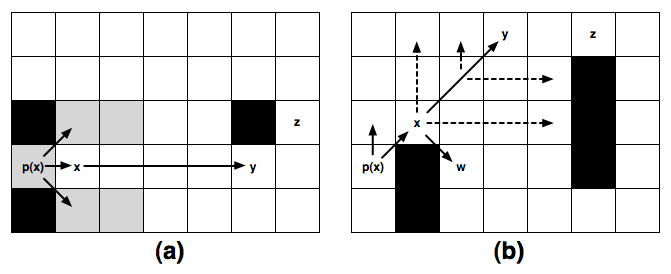
\includegraphics[width=0.95\columnwidth, trim = 10mm 10mm 10mm 0mm]
			{diagrams/jumppoints.png}
       \end{center}
	\vspace{-3pt}
       \caption{Examples of straight (a) and diagonal (b) jump points.
Dashed lines indicate a sequence of interim node evaluations that reached
a dead end. Strong lines indicate eventual successor nodes.}
       \label{fig:jumppoints}
\end{figure}

Here the search is expanding a node $x$ which has as its parent $p(x)$;
the direction of travel from $p(x)$ to $x$ is a straight move to the right.
When expanding $x$ we may notice that there is little point to evaluating any
neighbour highlighted grey as the path induced by such a move is always
dominated by (i.e. no better than) an alternative path which mentions 
$p(x)$ but not $x$.
We will make this idea more precise in the next section but for now it is 
sufficient to observe that the only non-dominated neighbour of $x$ 
lies immediately to the right.
Rather than generating this neighbour and adding it to the open list,
as in the classical A* algorithm, we propose 
to simply step to the right and continue moving in this direction until we
encounter a node such as $y$; which has at least one other non-dominated
neighbour (here $z$). 
If we find a node such as $y$ (a jump point) we generate it as a successor 
of $x$ and assign it a $g$-value (or cost-so-far) of $g(y) = g(x) + d(x,
y)$.
Alternatively, if we reach an obstacle we conclude that further search in this
direction is fruitless and generate nothing.
\par
In the remainder of this section we will develop a macro-step operator which 
speeds up node expansion by identifying jump point successors in the case of
both straight and diagonal moves. First it will be necessary to define a series of
pruning rules to determine whether a node should be generated 
or skipped. 
This will allow us to make precise the notion of a jump point and 
give a detailed description of the jump points algorithm.
Then, we prove that the process of ``jumping'' nodes, such as $x$ in 
Figure \ref{fig:jumppoints}(a), has no effect on the optimality of search.


\input pruning
\input jumpdesc
\input optimality

